%  $Description: Author guidelines and sample document in LaTeX 2.09$
%
%  $Author: ienne $
%  $Date: 1995/09/15 15:20:59 $
%  $Revision: 1.4 $
%
%\documentclass[times, 10pt,twocolumn]{article}
%\documentclass[conference,final]{IEEEtran}
\documentclass[10pt,conference]{IEEEtran}
\usepackage{latex8}
\usepackage{times}

% Users' option
\usepackage{amssymb}
\usepackage{amsmath}
\usepackage{graphicx}
\usepackage{epstopdf}
\usepackage{color}
\topmargin=0.01in
\usepackage{multirow}
\usepackage{booktabs}
\newif\ifdraft
\drafttrue

\renewcommand{\multirowsetup}{\centering}
\renewcommand{\arraystretch}{1.2}
\def\nyc{\centering}

\ifdraft
\newcommand{\fixme}[1]{ { \bf{ ***FIXME: #1 }} }
\newcommand{\jhanote}[1]{ {\textcolor{red} { ***Jha: #1 }}}
\newcommand{\Nkimnote}[1]{ {\textcolor{green} { ***Nkim: #1 }}}
\newcommand{\skonote}[1]{ {\textcolor{blue} { ***Jeff: #1 }}}
\else
\newcommand{\jhanote}[1]{}
\newcommand{\Nkimnote}[1]{}
\newcommand{\fixme}[1]{}
\newcommand{\skonote}[1]{}
\fi
% End of users' option

%\documentstyle[times,art10,twocolumn,latex8]{article}

%-------------------------------------------------------------------------
% take the % away on next line to produce the final camera-ready version
\pagestyle{empty}

\newcommand{\up}{\vspace*{-1em}}
\newcommand{\upp}{\vspace*{-0.5em}}
\newcommand{\ts}{$T_{s}$}


%-------------------------------------------------------------------------
\title{A Framework for Coupled Multi-physics Simulations \skonote{some charming title?? 
emphasizing ''it can cover various kinds of applications in different requirement, 
main components can be replaced by other similar softwares, etc.''} }

\author{
 ~\\[-2em]
 Soon-Heum Ko$^{1,2}$, Nayong Kim$^{2}$, Shantenu Jha$^{3,2}$\\
 \small{\emph{$^{1}$National Supercomputing Centre, Lin\"{o}ping University, Lin\"{o}ping, Sweden}}\\
 \small{\emph{$^{2}$Center for Computation \& Technology, Louisiana State University, USA}}\\
 \small{\emph{$^{3}$Dept. of Elec. and Comp. Eng., Rutgers University, Piscataway, New Jersey, USA}}\\
% \small{\emph{$^{*}$Contact Author}}\\
}

%\thispagestyle{empty}

\begin{document}

\maketitle

\begin{abstract}
we design and develop a multi-physics framework for coupled simulations
in which scientific components (codes) are logically separated.
Designed framework provides the interface between scientific components,
(compilation system for system architectures,)
a runtime environment for scheduling of coupled tasks, and
data management/code versioning support.
The framework is built by developing the data exchange interface 
between coupled codes, (providing the wrapping script to users' Makefiles,)
adopting a BigJob abstraction, and using the PetaShare service.
We apply this framework into the hybrid computational fluid dynamics -
particle dynamics application to demonstrate its capability.
\end{abstract}
\up\up

%-------------------------------------------------------------------------
\section{Introduction and Motivation}

''Coupled scientific simulations'' will refer to the scientific 
research procedure which involves the data exchange between
different components (either in parallel or in tandem). In both cases,
whether scientific tools are continuously exchanging the information 
during a single run or individual tools iteratively give the feedback
to their counterparts, scheduling the overall procedure and
providing the data stream under the distributed computing infrastructure
is a headache to domain scientists. It motivates the development of
a framework for coupled multi-component applications,
which provides the following capabilities:
%{\it Framework} is defined as ''an abstraction in which software 
%providing generic functionality can be selectively changed 
%by user code, thus providing application specific software.''~\cite{Framework}
%According to this definition, a coupled multi-component framework
%shall provide the following functionalities: 
(1) the framework provides the data interface between users' tools,
(2) embedded softwares should be adaptive to users' implementations 
in diverse formulations, and 
(3) they should be removable/replaceable by users' preferences.

Two types of formulations can be present on a coupled multi-component 
framework. One is to modularize all components and bind into
a single executable, and the other is to make multiple standalone softwares
and provide the interface between individual executable. 
The former is good for scheduling on most batch queue system and 
effectively using allocated resources, while some restrictions 
on data structure or standard grammar may apply on users' codes.
Also, the binary can be heavier to contain unused or non-optimized functions
for specific targets. The other gives much freedom in writing 
the individual component but can cause computational headache in scheduling
components in the remote production system.
We consider that binding into the single binary is recommendable if
all software packages are tightly coupled together for a single task or
they share most memory allocations. It is preferred to provide
the interface and the scheduling function if those packages are
sequentially loaded or they have different code structures.
%This way is desirable if one simulation package is apparently lighter than the other or multiples of components are working together for a single application target, or all elements share a very similar data structure with variables or all elements can be scheduled in a sequential/tandem order on the simulation process. Cactus framework is one such example.

A runtime environment for a coupled multi-physics application
~\cite{CCGrid_Hybrid} has been developed previously. In this work,
two coupled yet logically distributed scientific softwares have been
effectively scheduled under the single batch queue allocation, 
by the use of a BigJob~\cite{saga_royalsoc} with the load balancing
capability incorporated. It demonstrated that a Pilot-job formulation
can ease the scheduling of a coupled application whose components are
hardly packaged into a single binary. However this runtime environment
lacks the reusability because it only provides the scheduling functionality
between already-coupled distributed application codes.

In this work, we design and develop a coupled multi-component framework.
Along with the runtime environment between logically separated components,
we also provide the standard interface between these components and
take care of the data management/versioning. The structure of
a coupled simulation framework is introduced in Sec.~\ref{sec:design}.
Specific softwares implemented in this framework are described in
Sec.~\ref{sec:implementation}. A coupled multi-physics application and
an experiment-computation integrated research procedure are presented
in Sec.~\ref{sec:experiment}. Recommendation for future work and 
conclusions are presented in Sec.~\ref{sec:futureworks} and
Sec.~\ref{sec:conclusion}.



% -------------------------------------------------------------------------
\section{Design of a Coupled Simulation Framework}
\label{sec:design}

\subsection{Requirements}
Multiple components in a coupled application is hard to be packaged 
into a single binary if 
(1) each component uses very different computational kernels 
or 
(2) a manual procedure is involved in one of components.
A hybrid computational fluid dynamics (CFD) - molecular dynamics (MD) 
simulation is an example whose data structures are completely different
so that it is fairly hard to incorporate into a single binary.
Another situation is occasionally observed when there is an iterative
feedback between a numerical simulation and the experimental measurement.
Most probably, the physical experiment involves the human labor
of changing specimen/mockup after the numerical investigation, 
which cannot be digitalized.
Figure~\ref{Fig:Overall_Flow} describes the procedure for 
these two multi-component simulations.


%%%%% FIGURE %%%%%
\begin{figure}[ht]
\centering
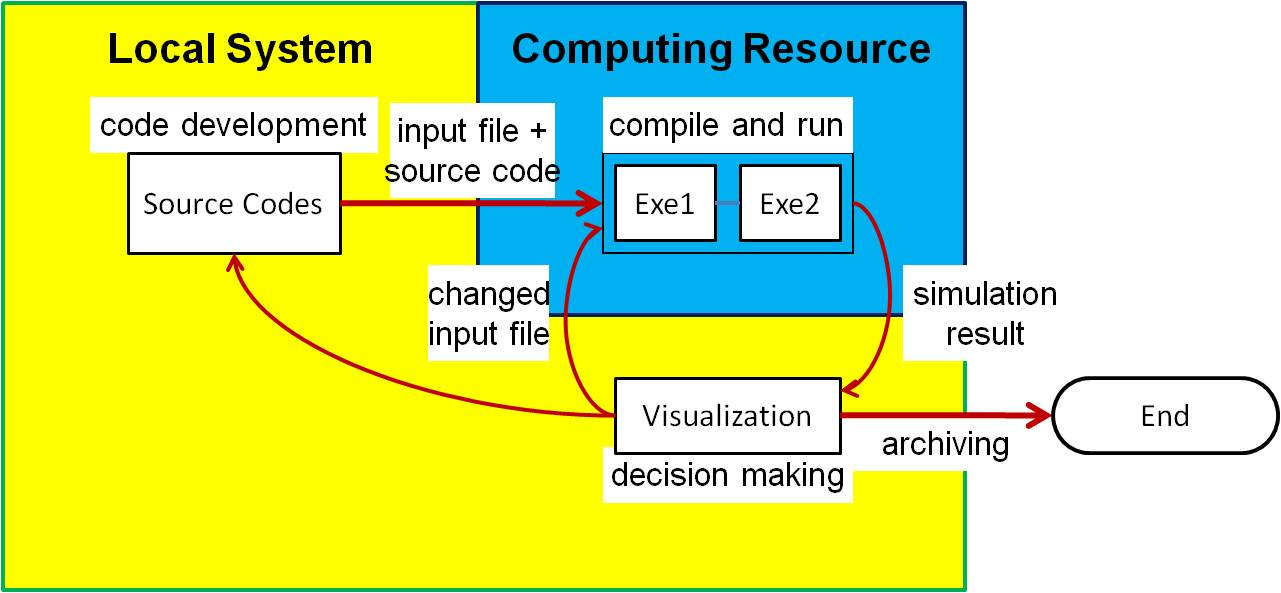
\includegraphics[width=0.8\linewidth]{Flow_Multiphysics_Simulation.jpg}
\vskip 0.2cm
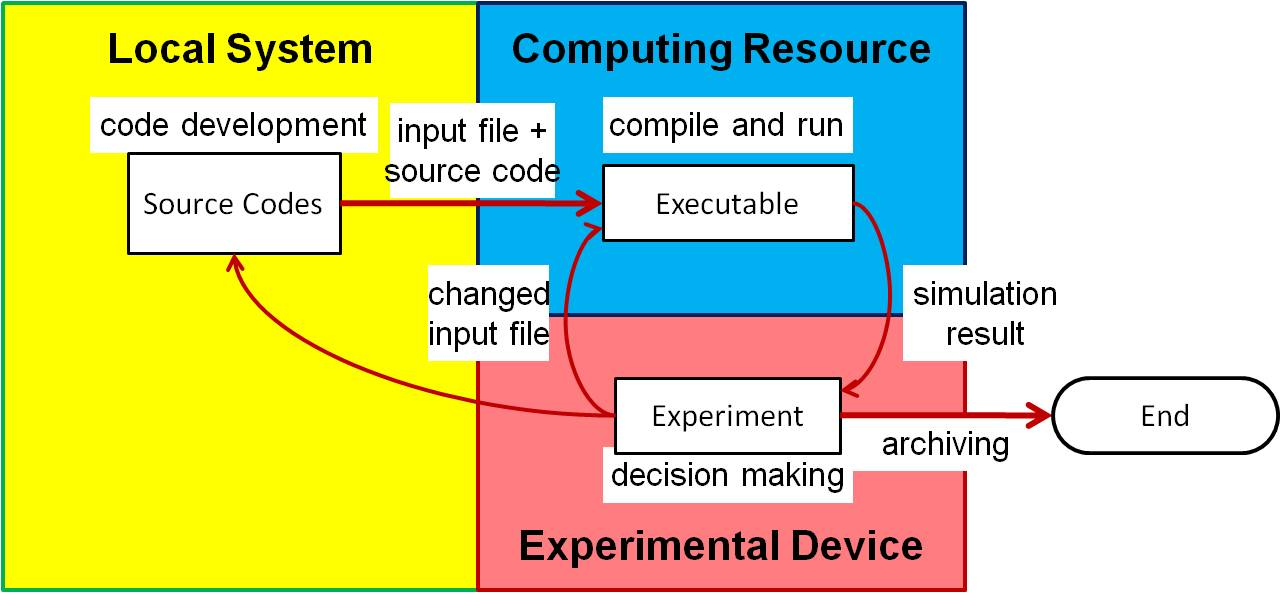
\includegraphics[width=0.8\linewidth]{Flow_Exp_and_Comp.jpg}
\vskip-0.2cm
\caption{\small {\bf Research procedure of 
(1) coupled multi-physics simulations and 
(2) successive feedback between computations and experiments.} 
In both cases, frequent data transfer takes place between 
local and remote systems and a manual decision making intervenes 
(either by visualizing the numerical solution or 
by performing the experimental measurement). In addition, 
the framework should support the communication interface and 
concurrent execution in case of computationally coupling 
distinct scientific softwares.}
\label{Fig:Overall_Flow}
\end{figure}
%%%%% FIGURE %%%%%


A coupled multi-component simulation framework should be capable of
scheduling the overall procedure (workflow) and
a coupled simulation between multiple tasks (runtime environment).
The workflow shall run software components according to 
the pre-described schedule, which includes scientific softwares 
and middleware packages. A runtime environment takes the role of
running coupled multiple softwares in parallel, 
in the form of a virtually single executable 
under the batch queue system.

The functionality to handle the data transfer/exchange provides
more convenience for performing the coupled simulation and 
building coupled software packages. Automated data transferring
eases the successive feedback between distributed tools,
and also provides the basic-level versioning service 
of source codes into the remote computing machines.
The coupling interface can take care of the synchronous communication
between concurrently running softwares.


\subsection{Design}
We design the concrete structure of a coupled multi-component 
simulation framework as presented in Fig.~\ref{Fig:Multicomponent_Framework}.
Looking at the default operation flow, the updated source code is copied to
the remote computing resource and the individual source code is linked with
the coupling interface during the compilation. These distinct yet coupled
executables run concurrently by the help of a runtime environment. The solution
is referenced by a third-party and the decision is made to accept/decline
the numerical solution (either through the visualization or 
the experimental measurement). The acceptable solution is archived 
in the local server, or the new computation is performed using different
parameter/modified source codes. In case the computation and 
the experimential measurement are coupled in sequence, 
compilation and job submission processes become simpler.


%%%%% FIGURE %%%%%
\begin{figure}[ht]
\centering
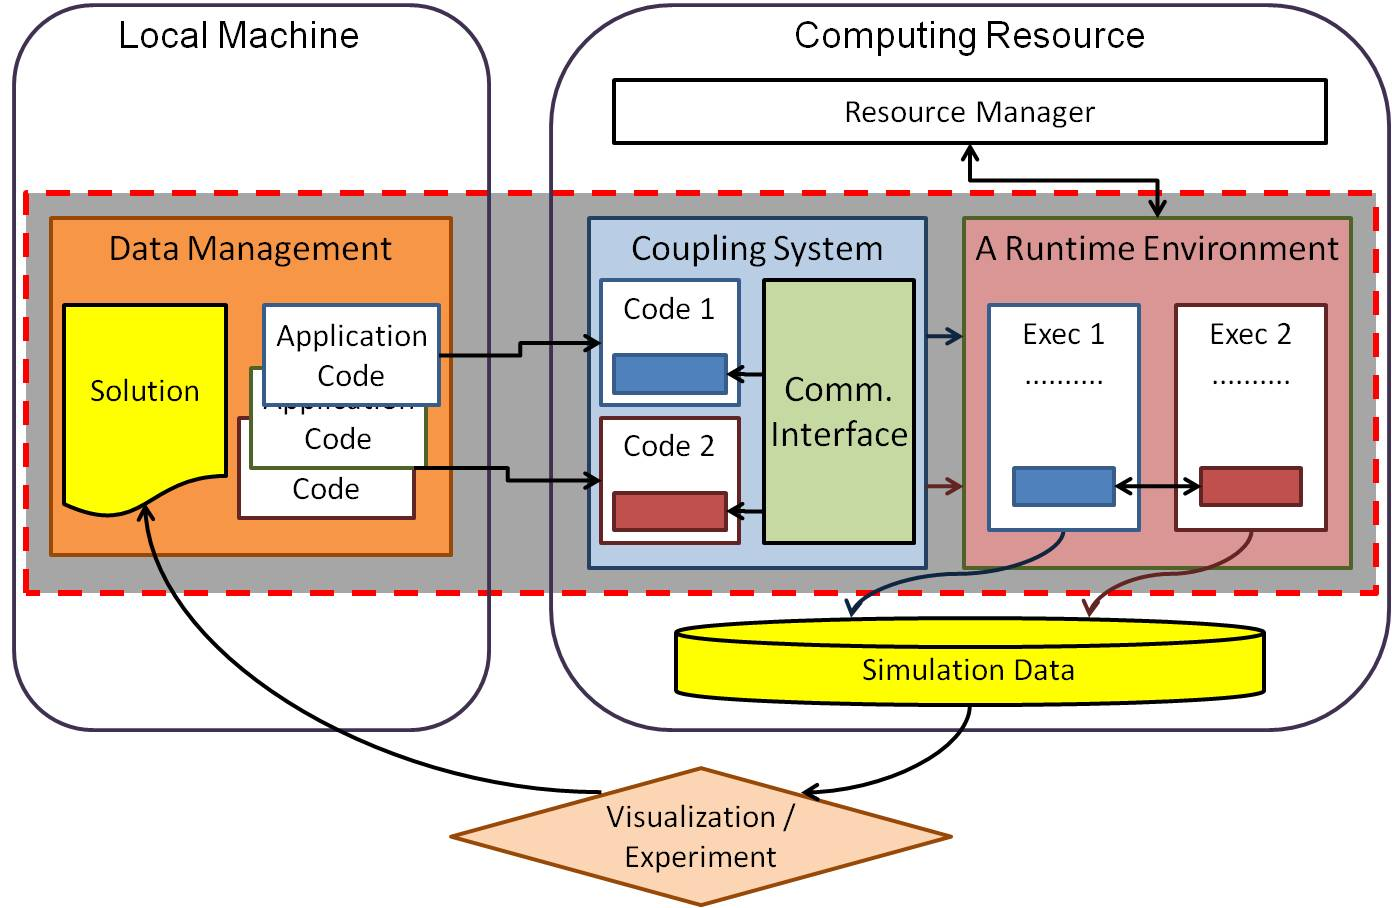
\includegraphics[width=0.8\linewidth]{Coupled_Framework_Diagram.jpg}
\vskip-0.2cm
\caption{\small {\bf Structure of a coupled multi-component application 
framework.} The framework is composed of three main packages: 
a data archiving/versioning service, a coupler and a runtime environment. 
A workflow script is running these packages according to the 
coupled simulation procedure.}
\label{Fig:Multicomponent_Framework}
\end{figure}
%%%%% FIGURE %%%%%


Data management service provides the data sharing among distributed computing
facilities, updating the source codes between local and remote machines, and
archiving final solutions. These functions can be implemented by running 
a couple of secure FTP commands;
Installing a versioning service such as 
CVS (Concurrent Versioning System:~\cite{CVS}), 
SVN (Apache Subversion:~\cite{SVN}), or 
GIT (The fast version control system:~\cite{GIT})
on a central repository server is another way; Using a data Grid service
such as PetaShare~\cite{PetaShare} can be helpful if sharing large-scale
data on a distributed environment is of particular interest.

Coupling system provides the data exchange between distinct application codes
and helps the compiling procedure. The coupling interface can be supported
either in the form of a library which opens a file-based channel between
distributed executables, or as a separate binary which binds all MPI
communicators under a single MPI runtime environment. In either case,
the interface function calls should be deployed in coupled source codes.
Compilation system handles all compilations including individual source
codes and the coupler. It wraps up compiling options on users' makefiles
to link the coupling library with the executable and 
to apply optimal options for specific systems. A single wrap-up script
can provide these capabilities up to some extent; Some compilation systems
such as the Simulation Factory~\cite{SimFactory} can provide more generality
independent of different system architectures and configurations.

A runtime environment is designed to co-schedule and load-balance between
coupled distinct tasks. The above issue is easily resolved by allocating
a pilot-job in which coupled subtasks are effectively scheduled. A number of
pilot-job implementations such as a Condor Glidein Job~\cite{Condor},
a BigJob~\cite{saga_royalsoc}, or a Pilot Factory~\cite{PilotFactory},
are present. Also, some supercomputing centers provide the capability of
concurrently starting multiple jobs in the basic level.

% -------------------------------------------------------------------------
\section{Implementation}
\label{sec:implementation}

\subsection{Data Management and Archiving}

\subsection{Coupling System}
- Library form (lighter), none-resource usage

\subsection{Runtime Environment}
We apply the previously-developed BigJob runtime environment for coupled
multi-physics applications~\cite{CCGrid_Hybrid}. The load balancing function
is turned off since it requires relevant changes (time checking function and
checkpointing capability) in the application code.
We directly submit a job to the remote batch queue system in case the
sequential feedback process between a computation and an experiment is
of interest.

\subsection{Workflow Engine}

% -------------------------------------------------------------------------
\section{Numerical Experiments}
\label{sec:experiment}

% -------------------------------------------------------------------------
\section{Further Achievements}
\label{sec:futureworks}

%-------------------------------------------------------------------------
\section{Conclusions}
\label{sec:conclusion}

%-------------------------------------------------------------------------
\section*{Acknowledgment}

%-------------------------------------------------------------------------
%\nocite{ex1,ex2}
\bibliographystyle{latex8}
%\bibliographystyle{IEEEtran}
\bibliography{saga_tg08}


\end{document}


